\documentclass[tikz,border=6pt]{standalone}
\usepackage{tikz}
\usepackage{amsmath}
\usetikzlibrary{arrows.meta,positioning,calc}
\begin{document}
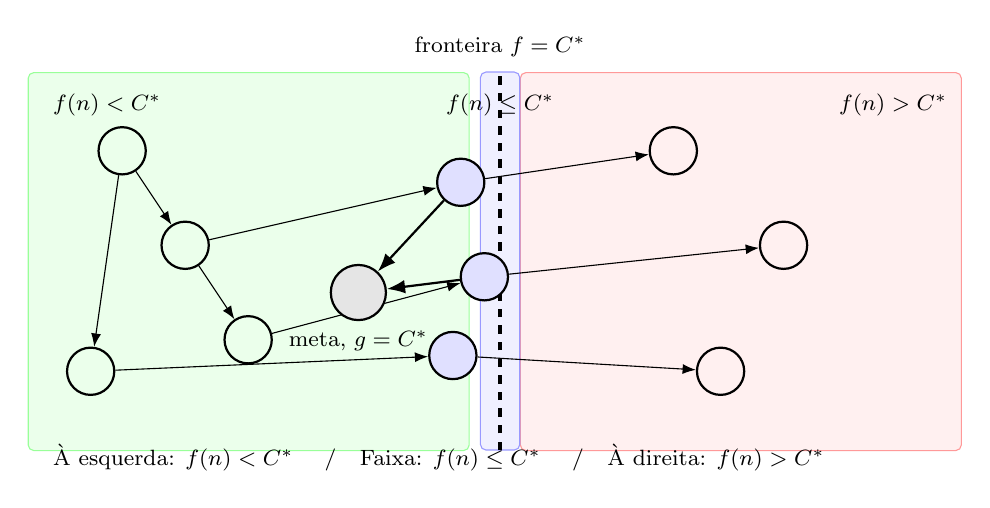
\begin{tikzpicture}[
  >=Latex,
  node/.style={circle, draw, thick, minimum size=6mm, inner sep=0pt},
  goal/.style={circle, draw, thick, fill=black!10, minimum size=7mm, inner sep=0pt},
  lab/.style={font=\footnotesize},
  regionL/.style={fill=green!8, draw=green!40, rounded corners=2pt},
  regionM/.style={fill=blue!6, draw=blue!40, rounded corners=2pt},
  regionR/.style={fill=red!6, draw=red!40, rounded corners=2pt}
]
\def\xL{-6} \def\xF{0} \def\xR{6}
\def\yT{2.6} \def\yB{-2.2} \def\gap{0.25}

\node[regionL, minimum width=5.6cm, minimum height=4.8cm, anchor=north west] at (\xL,\yT) {};
\node[regionR, minimum width=5.6cm, minimum height=4.8cm, anchor=north west] at (\xF+\gap,\yT) {};
\fill[regionM] (\xF-\gap,\yB) rectangle (\xF+\gap,\yT);

\draw[dashed, very thick] (\xF,\yB) -- (\xF,\yT);
\node[lab, above=2pt] at (\xF, \yT) {fronteira $f=C^*$};

\node[lab, anchor=north west] at (\xL+0.2, \yT-0.15) {$f(n)<C^*$};
\node[lab, anchor=north]     at (\xF, \yT-0.15)      {$f(n)\le C^*$};
\node[lab, anchor=north east] at (\xR-0.2, \yT-0.15) {$f(n)>C^*$};

\node[node] (a) at (-4.8, 1.6) {};
\node[node] (b) at (-4.0, 0.4) {};
\node[node] (c) at (-3.2,-0.8) {};
\node[node] (d) at (-5.2,-1.2) {};
\draw[->] (a) -- (b);
\draw[->] (b) -- (c);
\draw[->] (a) -- (d);

\node[node, fill=blue!12] (e) at (-0.5, 1.2) {};
\node[node, fill=blue!12] (f) at (-0.2, 0.0) {};
\node[node, fill=blue!12] (g) at (-0.6,-1.0) {};
\draw[->] (b) -- (e);
\draw[->] (c) -- (f);
\draw[->] (d) -- (g);

\node[node] (h) at (2.2, 1.6) {};
\node[node] (i) at (3.6, 0.4) {};
\node[node] (j) at (2.8,-1.2) {};
\draw[->] (e) -- (h);
\draw[->] (f) -- (i);
\draw[->] (g) -- (j);

\node[goal, label={[lab]below:$\text{meta},\, g=C^*$}] (goal) at (-1.8, -0.2) {};
\draw[->, thick] (e) -- (goal);
\draw[->, thick] (f) -- (goal);

\node[lab, align=center, anchor=north west] at (-5.8, \yB+0.2)
{À esquerda: $f(n)<C^*$ \quad/\quad Faixa: $f(n)\le C^*$ \quad/\quad À direita: $f(n)>C^*$};
\end{tikzpicture}
\end{document}
